\chapter{Release 1: Users, segmentation \& channels}

\phantomsection
\section*{Introduction}
In this chapter, we focus on the first release of our product, this release aims to create and enhance
the user experience, implement userbase segmentation strategies, and manage notification channels.
We will delve into the sprints backlog, design considerations, and the implementation process
undertaken to bring these features to fruition.

\addcontentsline{toc}{section}{Introduction}

\section{Sprints backlog}
During the Sprint Planning event, we estimated the effort required for each item in the first and second
sprints backlog based on the number of working hours.

The priority of backlog items is reflected by their relative order in the table. Items positioned
higher in the table indicate a higher priority. \\

\begin{longtable}{ | m{0.08\textwidth}  | m{0.18\textwidth} | m{0.39\textwidth} | c | }
    \caption{Backlog of Sprint 1 \& 2}                                                                                                       \\
    \hline
    \textbf{Sprint}         & \textbf{Epic}                                       & \textbf{User story}        & \textbf{Estimation (hours)} \\
    \hline
    \endfirsthead
    \hline
    \textbf{Sprint}         & \textbf{Epic}                                       & \textbf{User story}        & \textbf{Estimation (hours)} \\
    \hline
    \endhead
    \hline
    \endfoot
    \endlastfoot
    \multirow[t]{3}{5em}{1} & Authentication                                      & Authenticate               & 16                          \\

    \cline{2-4}
                            & \multirow{4}{5em}{Agents management}                & Create an agent            & 16                          \\
    \cline{3-4}
                            &                                                     & List agents                & 16                          \\
    \cline{3-4}
                            &                                                     & Edit an agent              & 8                           \\
    \cline{3-4}
                            &                                                     & Delete an agent            & 8                           \\
    \cline{2-4}
                            & \multirow{4}{5em}{Users management}                 & Create a notification user & 16                          \\
    \cline{3-4}
                            &                                                     & List notification users    & 16                          \\
    \cline{3-4}
                            &                                                     & Edit a notification user   & 8                           \\
    \cline{3-4}
                            &                                                     & Delete a notification user & 8                           \\
    \hline
    \multirow[t]{2}{5em}{2} & \multirow{4}{5em}{Audience management}              & Create an audience         & 24                          \\
    \cline{3-4}
                            &                                                     & List audiences             & 16                          \\
    \cline{3-4}
                            &                                                     & Edit an audience           & 8                           \\
    \cline{3-4}
                            &                                                     & Delete an audience         & 8                           \\
    \cline{2-4}
                            & \multirow{4}{5em}{Notification channels management} & Create a channel           & 32                          \\
    \cline{3-4}
                            &                                                     & List channels              & 16                          \\
    \cline{3-4}
                            &                                                     & Edit a channel             & 8                           \\
    \cline{3-4}
                            &                                                     & Delete a channel           & 8                           \\
    \hline
\end{longtable}

\section{Specification}
In this section we are going to provide a detailed breakdown of some user stories. Each user story will
be presented in a structured table format, ensuring ease of reference for the development
team and that each user story is comprehensively documented. This table will include four key components:

\begin{itemize}
    \item \textbf{Precondition:} Highlights any necessary conditions or prerequisites that must be
          in place before the user story can be initiated.
    \item \textbf{Business rules:} Business rules are critical as they define the constraints, policies,
          and conditions that govern how the software should behave in response to user interactions.
    \item \textbf{Technical specification:} This part specifies the technical aspects of the user story.
          It outlines the specific technical requirements, technologies, and architecture considerations that
          will be essential for the development team to realize the user story.
    \item \textbf{Acceptance criteria:} This section will provide a clear list of conditions that must
          be met for the user story to be considered complete and ready for release.
\end{itemize}


\begin{longtable}{ | m{0.2\textwidth} | m{0.75\textwidth} | }
    \caption{User stories specification}                                                                                                                                                                                                                                  \\
    \hline
    \textbf{Epic}                                      & \textbf{User story}                                                                                                                                                                                              \\
    \hline
    \endfirsthead
    \hline
    \textbf{Epic}                                      & \textbf{User story}                                                                                                                                                                                              \\
    \hline
    \endhead
    \endfoot
    \endlastfoot
    Authentication                                     & \textbf{Authenticate} \newline As a registered user, I want to be able to log into my account securely using my email and password.

    \paragraph*{Precondition} \mbox{} \newline
    \begin{itemize}
        \item User is already registered and has a valid account.
    \end{itemize}

    \paragraph*{Business rules} \mbox{} \newline
    \begin{itemize}
        \item Users must provide an email and password to authenticate.
        \item Users should not be able to authenticate if credentials are incorrect.
        \item Users must be redirected to the page they were trying to access before being prompted to log in.
        \item Users must be able to reset their passwords if they forget them.
    \end{itemize}
    \paragraph*{Technical specification} \mbox{} \newline
    \begin{itemize}
        \item The email field should accept a valid email address.
        \item The login form should include a "Forgot Password" link that allows the user to reset their password.

    \end{itemize}
    \paragraph*{Acceptance criteria} \mbox{} \newline
    \begin{itemize}
        \item User email and password are both required for log in.
        \item Users should be able to log in using their registered email and password.
        \item Invalid login attempts should result in an error message.
    \end{itemize}                                                                                                                                                                                        \\
    \hline
    Notification users management                      & \textbf{Create a notification user} \newline As an administrator/agent, I want to be able to create users so that I can send them notifications.
    \paragraph*{Precondition} \mbox{} \newline
    \begin{itemize}
        \item Administrator/Agent authenticated and has a valid account.
        \item Users do not exist already
    \end{itemize}
    \paragraph*{Business rules} \mbox{} \newline
    \begin{itemize}
        \item Creation form should include a first and last name, email, a phone number,
              a birthdate, a language key and a country.
        \item Administrators/Agents should be able to download a file containing the data format
              to respect when importing users from a file.
        \item Administrators/Agents shouldn’t be able to add a user with an already existing
              email or phone number.
        \item Administrators/Agents should be able to import a list of users from a file.
    \end{itemize}
    \paragraph*{Technical specification} \mbox{} \newline
    \begin{itemize}
        \item The email field should accept a valid email address.
        \item The phone number field should accept a valid phone number.
        \item File import should accept only \acrshort{csv} files.
    \end{itemize}
    \paragraph*{Acceptance criteria} \mbox{} \newline
    \begin{itemize}
        \item All required fields are provided: first and last name, email or phone number, and the country.
        \item Created or imported users are saved to the database.
        \item A message indicating the success or failure of the operation is displayed.
    \end{itemize}                                                                                                                                                                   \\
    \hline
    Notification \newline channels \newline management & \textbf{Create a notification channel} \newline As an administrator, I want to be able to create notification channels so that agents can use them to send notifications.
    \paragraph*{Precondition} \mbox{} \newline
    \begin{itemize}
        \item Administrator is authenticated and has a valid account.
    \end{itemize}
    \paragraph*{Business rules} \mbox{} \newline
    \begin{itemize}
        \item Each notification channel must have a unique name.
        \item The administrator should choose the type of notification channel, such as email, SMS, or push notifications.
        \item The administrator should be able to configure the desired provider for the chosen channel type.
    \end{itemize}
    \paragraph*{Technical specification} \mbox{} \newline
    \begin{itemize}
        \item A form should be provided for the administrator to enter the channel's name, type, the provider and its configuration.
        \item The system should be able to handle multiple types of service providers, each with their own configurations.
        \item The service provider credentials should be stored securely in the database.
        \item The system should be able to integrate with external service providers using APIs.
              % \item An API should be created to allow other parts of the system to send notifications through the notification channels.
    \end{itemize}
    \paragraph*{Acceptance criteria} \mbox{} \newline
    \begin{itemize}
        \item The administrator can successfully create a new notification channel.
        \item The administrator can conveniently configure the settings for each selected provider, such as API keys and credentials.
        \item The system is able to deliver the notifications through the created channel according to its configurations.
        \item A message indicating the success or failure of the operation is displayed.
    \end{itemize}                                                                                                                                          \\
    \hline
    Audience \newline management                       & \textbf{Create an audience} \newline As an administrator/agent, I want to be able to create a segment of user subscriptions based on some criteria, so that I can target these subscriptions with notifications.
    \paragraph*{Precondition} \mbox{} \newline
    \begin{itemize}
        \item Administrator/Agent is authenticated and has a valid account.
        \item Existing notification users and subscriptions.
    \end{itemize}
    \paragraph*{Business rules} \mbox{} \newline
    \begin{itemize}
        \item Administrators/Agents should be able to create a segment based on one or more criteria including subscription channel, language, country, age, or other user or subscription attributes.
        \item Administrators/Agents should be able to create as many audiences as they need.
        \item Administrators/Agents should be able to store and retrieve audience data from the database.
        \item Administrators/Agents should be able to get an estimation of the audience size while creation.
    \end{itemize}
    \paragraph*{Technical specification} \mbox{} \newline
    \begin{itemize}
        \item A user subscription can be part of multiple audiences at the same time.
        \item An audience shouldn't be empty, and should contain at least one notification subscription.
        \item Administrators/Agents can create multiple audiences with different criteria.
    \end{itemize}
    \paragraph*{Acceptance criteria} \mbox{} \newline
    \begin{itemize}
        \item The audience name should be unique.
        \item Administrators/Agents can create an audience based on at least one criteria.
        \item The group should only contain users satisfying the specified selection criteria.
        \item A message indicating the success or failure of the operation is displayed.
    \end{itemize}                                                                                                                                                                                 \\
    \hline
\end{longtable}

\section{Design}
The design phase of software development is a critical step in the software development life cycle.
It is the process of transforming the customer requirements into a detailed plan for how the software
will be implemented. In this section we are going to focus on the design aspects related to the software
and database design.

\subsection{Class diagram}
The class diagram provides a high-level overview of the system's structure, relationships,
and interactions between different classes. It represents the static structure of the system,
including classes, attributes, methods, and associations.

\noindent The following table provides a description of each class being part of the first release design.

\begin{longtable}{ | m{0.3\textwidth} | m{0.645\textwidth} | }
    \caption{Classes description}                                                                                                               \\
    \hline
    \textbf{Class name}      & \textbf{Description}                                                                                             \\
    \hline
    \endfirsthead
    \hline
    \textbf{Class name}      & \textbf{Description}                                                                                             \\
    \hline
    \endhead
    \endfoot
    \hline
    \endlastfoot
    User                     & This class represents the user entity in our solution                                                            \\
    \hline
    Authority                & This class represents roles which are going to be assigned to users                                              \\
    \hline
    NotificationUser         & This class represents the target customers for receiving notifications                                           \\
    \hline
    Channel                  & This class represents the notification channels that are going to send notifications through to our target users \\
    \hline
    ServiceProvider          & This class models the credentials of the third party service to integrate with the channel                       \\
    \hline
    NotificationSubscription & This class models a user notification subscription to a specific notification channel                            \\
    \hline
    Audience                 & This class models a segment of notification user subscriptions selected based on a criteria                      \\
    \hline
    Criteria                 & This class models a selection criteria for an audience, it represents a filter, an operator, and a value         \\
\end{longtable}


\noindent The figure \ref{r1-class} illustrates the class diagram for our first release. \\


\begin{figure}[hbt!]
    \centering
    \includesvg[width=\textwidth]{diagrams/class/r1-classp}
    \caption{The class diagram of the first release}
    \label{r1-class}
\end{figure}

\subsection{Database design}
In this section, We will discuss the structure and organization of our database, defining tables and relationships
between entities for efficient data management within our solution.

\subsubsection{Data dictionary}

First, we will define a data dictionary that describes the fields associated with each data element,
indicating their types and constraints as shown in the table \ref{tab-r1dd}.

\begin{landscape}
    \begin{longtable}{ | m{0.225\textwidth} | m{0.28\textwidth} | m{0.55\textwidth} | m{0.15\textwidth} | m{0.2\textwidth} | }
        \caption{Data dictionary of the first release}    \label{tab-r1dd}                                                                                                                                                                                                                 \\
        \hline
        \textbf{Entity}                                                  & \textbf{Field}                            & \textbf{Description}                                                                                                & \textbf{Type} & \textbf{Constraints}          \\
        \hline
        \endfirsthead
        \hline
        \textbf{Entity}                                                  & \textbf{Field}                            & \textbf{Description}                                                                                                & \textbf{Type} & \textbf{Constraints}          \\
        \hline
        \endhead
        \hline
        \endfoot
        \endlastfoot
        \multirow[t]{8}{5em}{\textbf{User}}                              & \texttt{id}                               & User's unique identifier                                                                                            & bigint        & Primary key \newline Not null \\
        \cline{2-5}
                                                                         & \texttt{first\char`_name}                 & User's first name                                                                                                   & varchar(50)   &                               \\
        \cline{2-5}
                                                                         & \texttt{last\char`_name}                  & User's last name                                                                                                    & varchar(50)   &                               \\
        \cline{2-5}
                                                                         & \texttt{email}                            & User's email address                                                                                                & varchar(256)  & Unique, Not null              \\
        \cline{2-5}
                                                                         & \texttt{password\char`_hash}              & User's encrypted password string                                                                                    & varchar(60)   & Not null                      \\
        \cline{2-5}
                                                                         & \texttt{image}                            & User's profile image url                                                                                            & varchar(256)  &                               \\
        \cline{2-5}
                                                                         & \texttt{lang\char`_key}                   & User's prefered language key                                                                                        & varchar(10)   &                               \\
        \cline{2-5}
                                                                         & \texttt{avtivated}                        & User's account activation status                                                                                    & boolean       & Not null                      \\
        \hline
        \textbf{Authority}                                               & \texttt{name}                             & User authority (role)                                                                                               & varchar(50)   & Primary key                   \\
        \hline
        \multirow[t]{8}{5em}{\textbf{NotificationUser}}                  & \texttt{id}                               & Notification user unique identifier                                                                                 & bigint        & Primary key \newline Not null \\
        \cline{2-5}
                                                                         & \texttt{first\char`_name}                 & Notification user's first name                                                                                      & varchar(50)   & Not null                      \\
        \cline{2-5}
                                                                         & \texttt{last\char`_name}                  & Notification user's last name                                                                                       & varchar(50)   & Not null                      \\
        \cline{2-5}
                                                                         & \texttt{email}                            & Notification user's email address                                                                                   & varchar(256)  & Not null                      \\
        \cline{2-5}
                                                                         & \texttt{phone\char`_number}               & Notification user's phone number                                                                                    & varchar(50)   &                               \\
        \cline{2-5}
                                                                         & \texttt{lang\char`_key}                   & Notification user's prefered language key                                                                           & varchar(10)   & Not null                      \\
        \cline{2-5}
                                                                         & \texttt{country}                          & Notification user's country location                                                                                & varchar(256)  & Not null                      \\
        \cline{2-5}
                                                                         & \texttt{birth\char`_date}                 & Notification user's birth date                                                                                      & date          &                               \\
        \hline
        \multirow[t]{6}{5em}{\textbf{Channel}}                           & \texttt{id}                               & Notification channel's unique identifier                                                                            & bigint        & Primary key \newline Not null \\
        \cline{2-5}
                                                                         & \texttt{name}                             & Notification channel's name                                                                                         & varchar(100)  & Unique, Not null              \\
        \cline{2-5}
                                                                         & \texttt{channel\char`_type}               & Notification channel's type (EMAIL, SMS, PUSH, or CHAT)                                                             & varchar(10)   & Not null                      \\
        \cline{2-5}
                                                                         & \texttt{creation\char`_date}              & Notification channel's creation date                                                                                & datetime      &                               \\
        \cline{2-5}
                                                                         & \texttt{service\char`_provider\char`_id}  & Notification channel's specific service provider identifier                                                         & bigint        & Unique, Not null              \\
        \cline{2-5}
                                                                         & \texttt{creator\char`_id}                 & Identifier of the channel creator                                                                                   & bigint        & Unique, Not null              \\
        \hline
        \multirow[t]{13}{5em}{\textbf{ServiceProvider}}                  & \texttt{id}                               & Notification sending service provider's unique identifier                                                           & bigint        & Primary key \newline Not null \\
        \cline{2-5}
                                                                         & \texttt{provider\char`_id}                & Service provider name identifier                                                                                    & varchar(50)   & Not null                      \\
        \cline{2-5}
                                                                         & \texttt{host}                             & Host address for the \acrshort{smtp} mail server                                                                    & varchar(256)  &                               \\
        \cline{2-5}
                                                                         & \texttt{port}                             & Server port for the \acrshort{smtp} mail server                                                                     & integer       &                               \\
        \cline{2-5}
                                                                         & \texttt{encryption}                       & Encryption type for the \acrshort{smtp} mail server                                                                 & varchar(10)   &                               \\
        \cline{2-5}
                                                                         & \texttt{username}                         & Username for authenticating to the \acrshort{smtp} mail server                                                      & varchar(256)  &                               \\
        \cline{2-5}
                                                                         & \texttt{password}                         & Password for authenticating to the \acrshort{smtp} mail server                                                      & varchar(60)   &                               \\
        \cline{2-5}
                                                                         & \texttt{from}                             & The sender credential for the \acrshort{smtp} mail server or Twilio SMS provider                                    & varchar(256)  &                               \\
        \cline{2-5}
                                                                         & \texttt{identifier}                       & Generic identifier for the service provider                                                                         & varchar(256)  &                               \\

                                                                         & \texttt{token}                            & Access token for the service provider                                                                               & varchar(60)   &                               \\
        \cline{2-5}
                                                                         & \texttt{messaging\char`_service}          & Whether or not to use a messaging service for Twilio provider                                                       & boolean       &                               \\
        \cline{2-5}
                                                                         & \texttt{channel\char`_secret}             & Secret code for the Line chat provider channel                                                                      & varchar(60)   &                               \\
        \cline{2-5}
                                                                         & \texttt{service\char`_account}            & The whole configuration file content of the Firebase service account                                                & text          &                               \\
        \hline
        \multirow[t]{5}{5em}{\textbf{Notification \newline Subsciption}} & \texttt{id}                               & Notification user subscription unique identifier                                                                    & bigint        & Primary key \newline Not null \\
        \cline{2-5}
                                                                         & \texttt{enabled}                          & Whether the subscription is enabled or disabled                                                                     & boolean       & Not null                      \\
        \cline{2-5}
                                                                         & \texttt{device\char`_token}               & The user token used to send notifications through, could be an email address, phone number, social media identifier & varchar(256)  & Not null                      \\
        \cline{2-5}
                                                                         & \texttt{notification\char`_user\char`_id} & Subscription's user identifier                                                                                      & bigint        & Not null                      \\
        \cline{2-5}
                                                                         & \texttt{channel\char`_id}                 & Subscription's notification channel identifier                                                                      & bigint        & Not null                      \\
        \hline
        \multirow[t]{5}{5em}{\textbf{Audience}}                          & \texttt{id}                               & Audience's unique identifier                                                                                        & bigint        & Primary key \newline Not null \\
        \cline{2-5}
                                                                         & \texttt{name}                             & Audience name                                                                                                       & varchar(100)  & Unique, Not null              \\
        \cline{2-5}
                                                                         & \texttt{creation\char`_date}              & Audience's creation date                                                                                            & datetime      & Not null                      \\
        \cline{2-5}
                                                                         & \texttt{size\char`_estimate}              & Audience's size estimation                                                                                          & bigint        & Not null                      \\
        \cline{2-5}
                                                                         & \texttt{creator\char`_id}                 & Audience's creator identifier                                                                                       & bigint        & Not null                      \\
        \hline
        \multirow[t]{8}{5em}{\textbf{Criteria}}                          & \texttt{id}                               & Criteria's unique identifier                                                                                        & bigint        & Primary key \newline Not null \\

                                                                         & \texttt{filter}                           & The attribute used to filter out notification subscriptions                                                         & boolean       & Not null                      \\
        \cline{2-5}
                                                                         & \texttt{operator}                         & The operator used to create the comparison for the filter                                                           & varchar(20)   & Not null                      \\
        \cline{2-5}
                                                                         & \texttt{value}                            & The value to filter subscriptions by                                                                                & varchar(50)   & Not null                      \\
        \cline{2-5}
                                                                         & \texttt{audience\char`_id}                & The unique identifier of the audience to which this criteria belongs                                                & bigint        & Not null                      \\
        \hline
    \end{longtable}
\end{landscape}


\subsubsection{Logical data model}
A logical data model is a model that is not specific to a database that describes things about which
an organization wants to collect data, and the relationships among these things \cite{ldm}. It contains representations
of entities and attributes, relationships, unique identifiers, and constraints between relationships.  The goal
of creating a logical data model is to develop a highly technical map of underlying rules and data structures.

\noindent The figure \ref{r1-erd}  illustrates the entity-relationship diagram for our first release. \\


\begin{figure}[hbt!]
    \centering
    \includesvg[width=\textwidth]{diagrams/database/r1-erd}
    \caption{The Entity-Relationship diagram of the first release}
    \label{r1-erd}
\end{figure}


\subsection{Sequence diagrams}
In this section, we delve into the dynamic aspects of our software solution by employing \acrshort{uml}
sequence diagrams. These diagrams provide a visual representation of the interactions and communication
patterns among various components and actors within our system. As we explore these sequences,
we aim to shed light on the flow of information, the order of operations, and the coordination
between different elements in our software architecture.


\subsubsection{Sequence diagram for Creating a channel}
First, we outline the process of creating notification channels, a critical functionality
designed to integrate external notification delivery services within our solution.

As depicted in the user story, only administrators can create and manage channels. After filling the channel
credentials the client validates the input data at the component level and hands the request to
the server. In order to verify channel credentials, our server needs to communicate with external servers (Facebook,
Twilio, Slack, Line). The reponse then tells if the channel is valid and could be saved in the database,
or the credentials are invalid which cancels the request and asks the administrator to verify their input.

\noindent The following figure \ref{seq-create-channel} illustrates the sequence diagram for creating a channel.

\subsubsection{Sequence diagram for creating an audience}
For the user segmentation feature, both administrators and agents have the ability to create segments
based on specific criteria.  This essential functionality enables them to precisely target user subscriptions
with relevant notifications.

In order to create an audience, users (administrators or agents) need to give their new audiences a name,
then they can add one or more selection criteria while specifying for each criteria: a filter, a comparison operator,
and a filtering value. The service layer of the client intercepts the changes while users are adding these criteria
to make audience size estimation requests to the server, updating this information every short interval of time
to keep users informed about the segments they are creating.

\noindent The following figure \ref{seq-create-audience} illustrates the sequence diagram for creating an audience.

\begin{landscape}
    \begin{figure}[hbt!]
        \centering
        \includesvg[width=1.55\textwidth]{diagrams/sequence/seq-create-channel}
        \caption{Sequence diagram for Creating a Channel}
        \label{seq-create-channel}
    \end{figure}
\end{landscape}

\begin{landscape}
    \begin{figure}[hbt!]
        \centering
        \includesvg[width=1.55\textwidth]{diagrams/sequence/seq-create-audience}
        \caption{Sequence diagram for creating an audience}
        \label{seq-create-audience}
    \end{figure}
\end{landscape}


\section{Implementation}
In the following section, we embark on a visual journey through a series of captured screenshots to provide
an in-depth glimpse into the user interface and functionality of our application.
the implementation of our application.

\subsection{Authentication}
The figure \ref{ss-signin} showcases the live implementation of the sign-in page, where users can provide
their credentials (email address and password) in order to authenticate. The "Remember Me" checkbox allows
users to stay signed in on future visits without the need to re-enter their credentials. The "Forget your
password?" link provides a way for users to reset their password if they have forgotten it, and if there's
an authentication error, a red banner with the error message is displayed above the input fields. \\

\begin{figure}[hbt!]
    \centering
    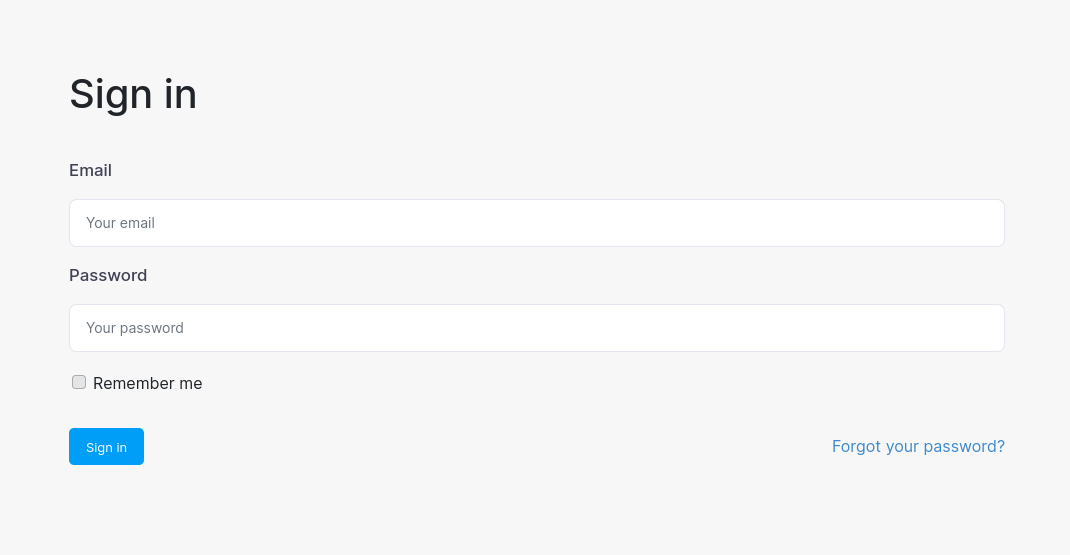
\includegraphics[width=\textwidth]{app/signin}
    \caption{Authentication page}
    \label{ss-signin}
\end{figure}


The figure \ref{ss-reset} illustrates the implementation of the reset password page. A user is redirected to
this interface when they click on the "Forgot your password?" link from the previous "Sign In" page,
they should provide their email address and click on the reset button. A banner indicating that an email
to recover their password is sent to their email address shows above the email input field.
\begin{figure}[hbt!]
    \centering
    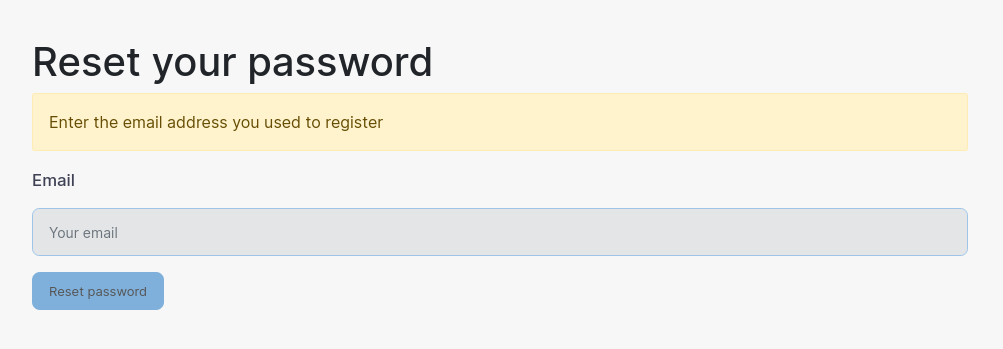
\includegraphics[width=\textwidth]{app/reset}
    \caption{Password reset page}
    \label{ss-reset}
\end{figure}

\subsection{Agents management}
The figure \ref{ss-agents} illustrates the implementation of the agents management page.
The table lists all the users (agents and administrators) for the logged in administrator, showing
an overview of their information. For each user, an administrator can edit, reset a password, or delete
an agent using the action buttons in the most right column, or else they can create a new
agent or administrator using the "Create a new agent" button.

\begin{figure}[hbt!]
    \centering
    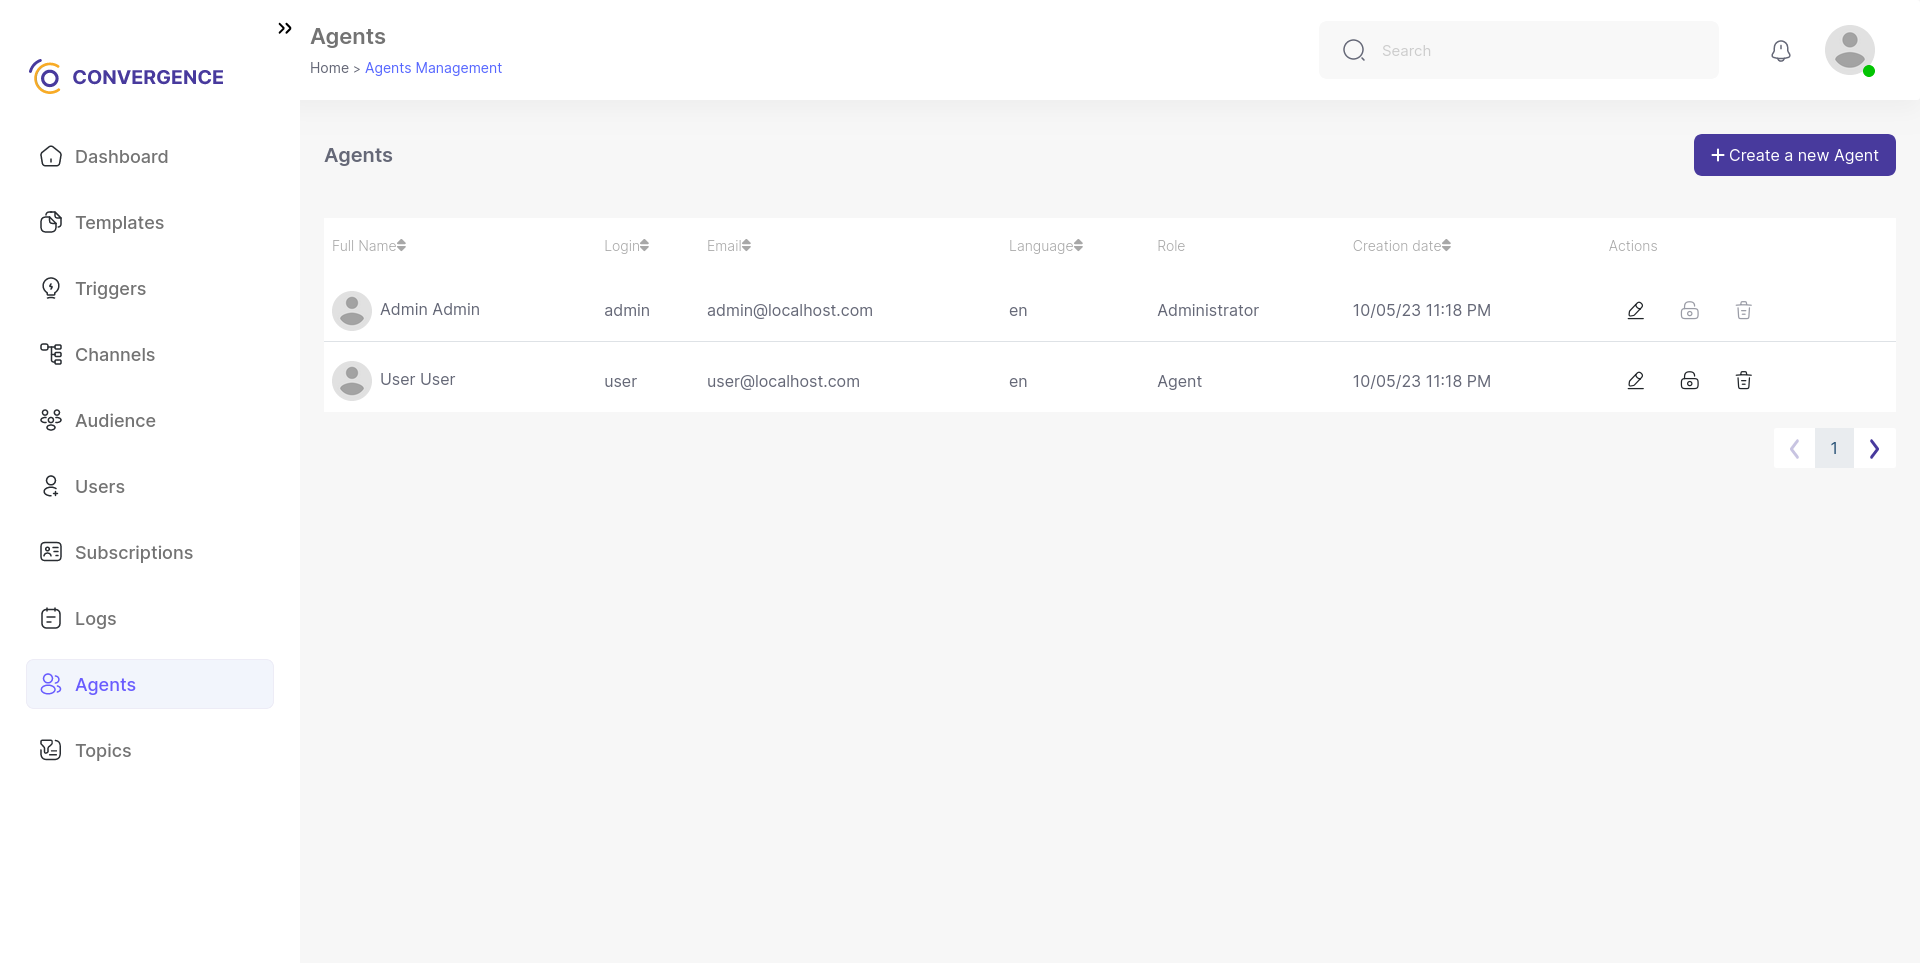
\includegraphics[width=\textwidth]{app/agents}
    \caption{Agents management page}
    \label{ss-agents}
\end{figure}

\subsection{Channels management}
The figure \ref{ss-channels} illustrates the final result of the implementation of channels management. The table
lists information about created channels for every service provider that can integrate with our solution. The
administrator can edit or delete these channels using the action buttons.
\begin{figure}[hbt!]
    \centering
    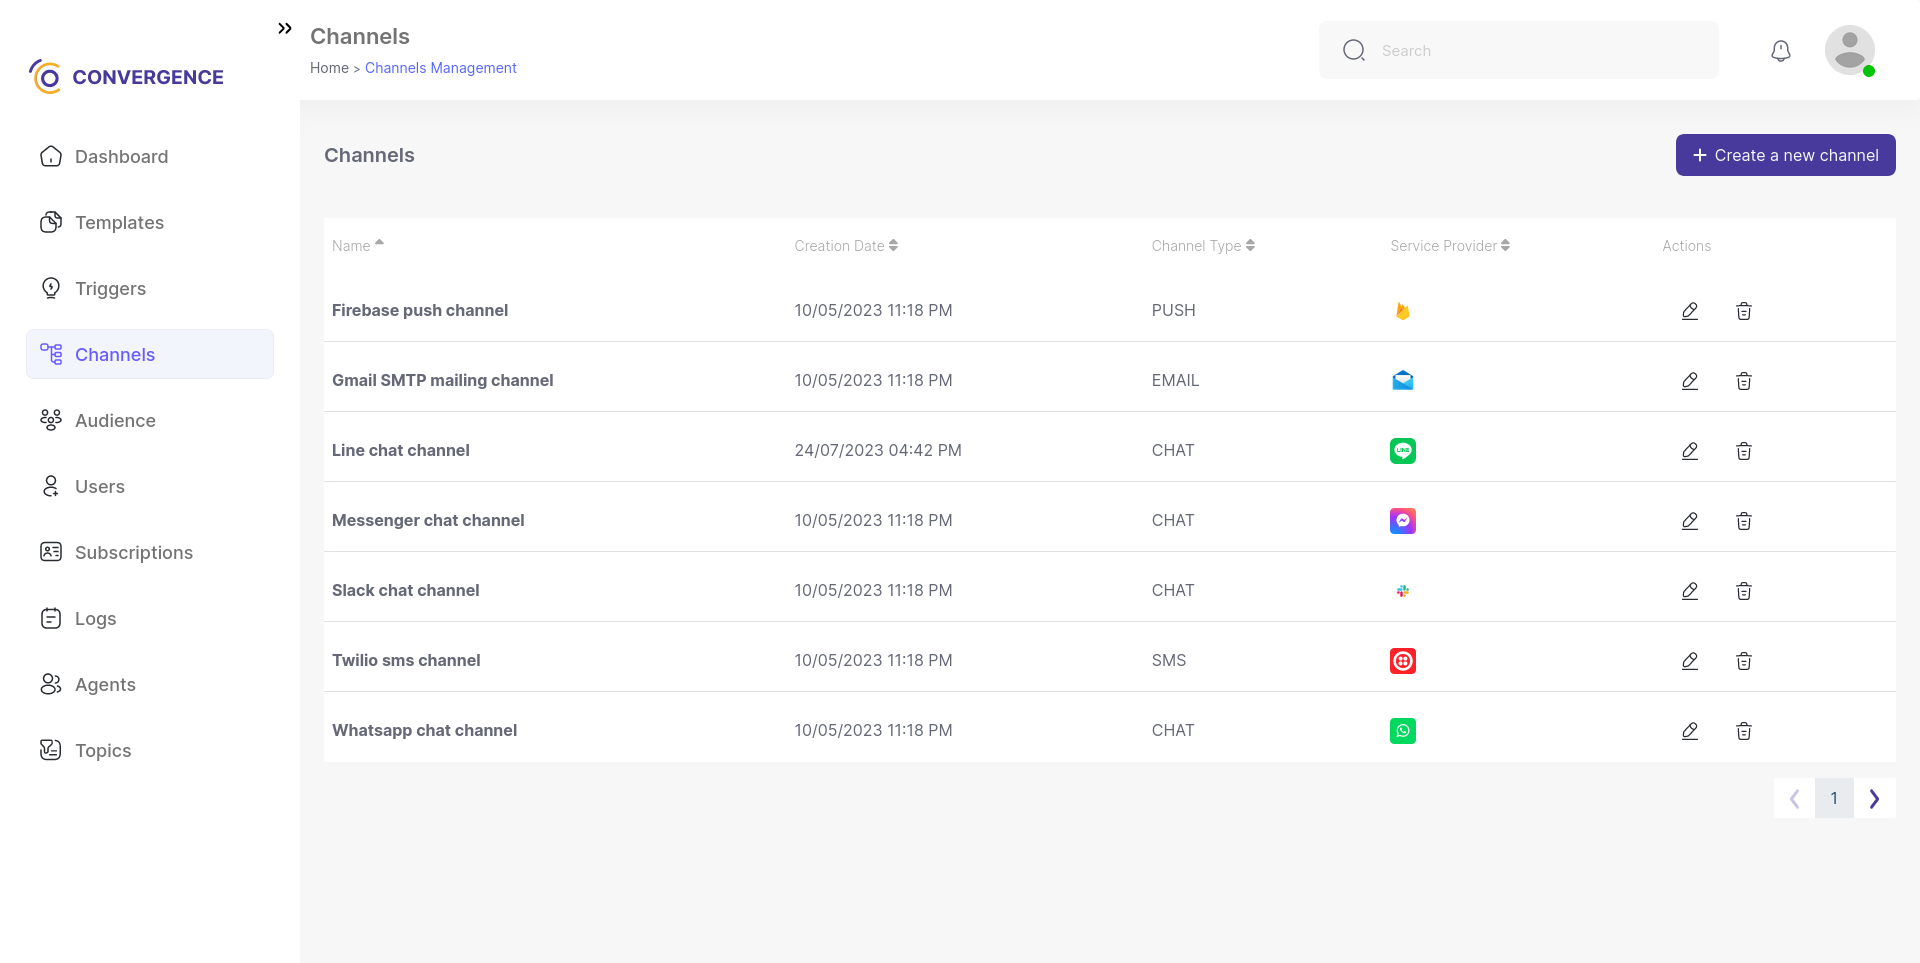
\includegraphics[width=\textwidth]{app/channels}
    \caption{Channels management page}
    \label{ss-channels}
\end{figure}

\subsection{Audience management}
The figure \ref{ss-audience} illustrates the final result of the implementation of the audience creation page.
We created some selection criteria: the subsciption channel should be of email type, users age should be greater
than 18 years, and subscribers are located in Tunisia. The size estimation for such audience is displayed in the section above.
\begin{figure}[hbt!]
    \centering
    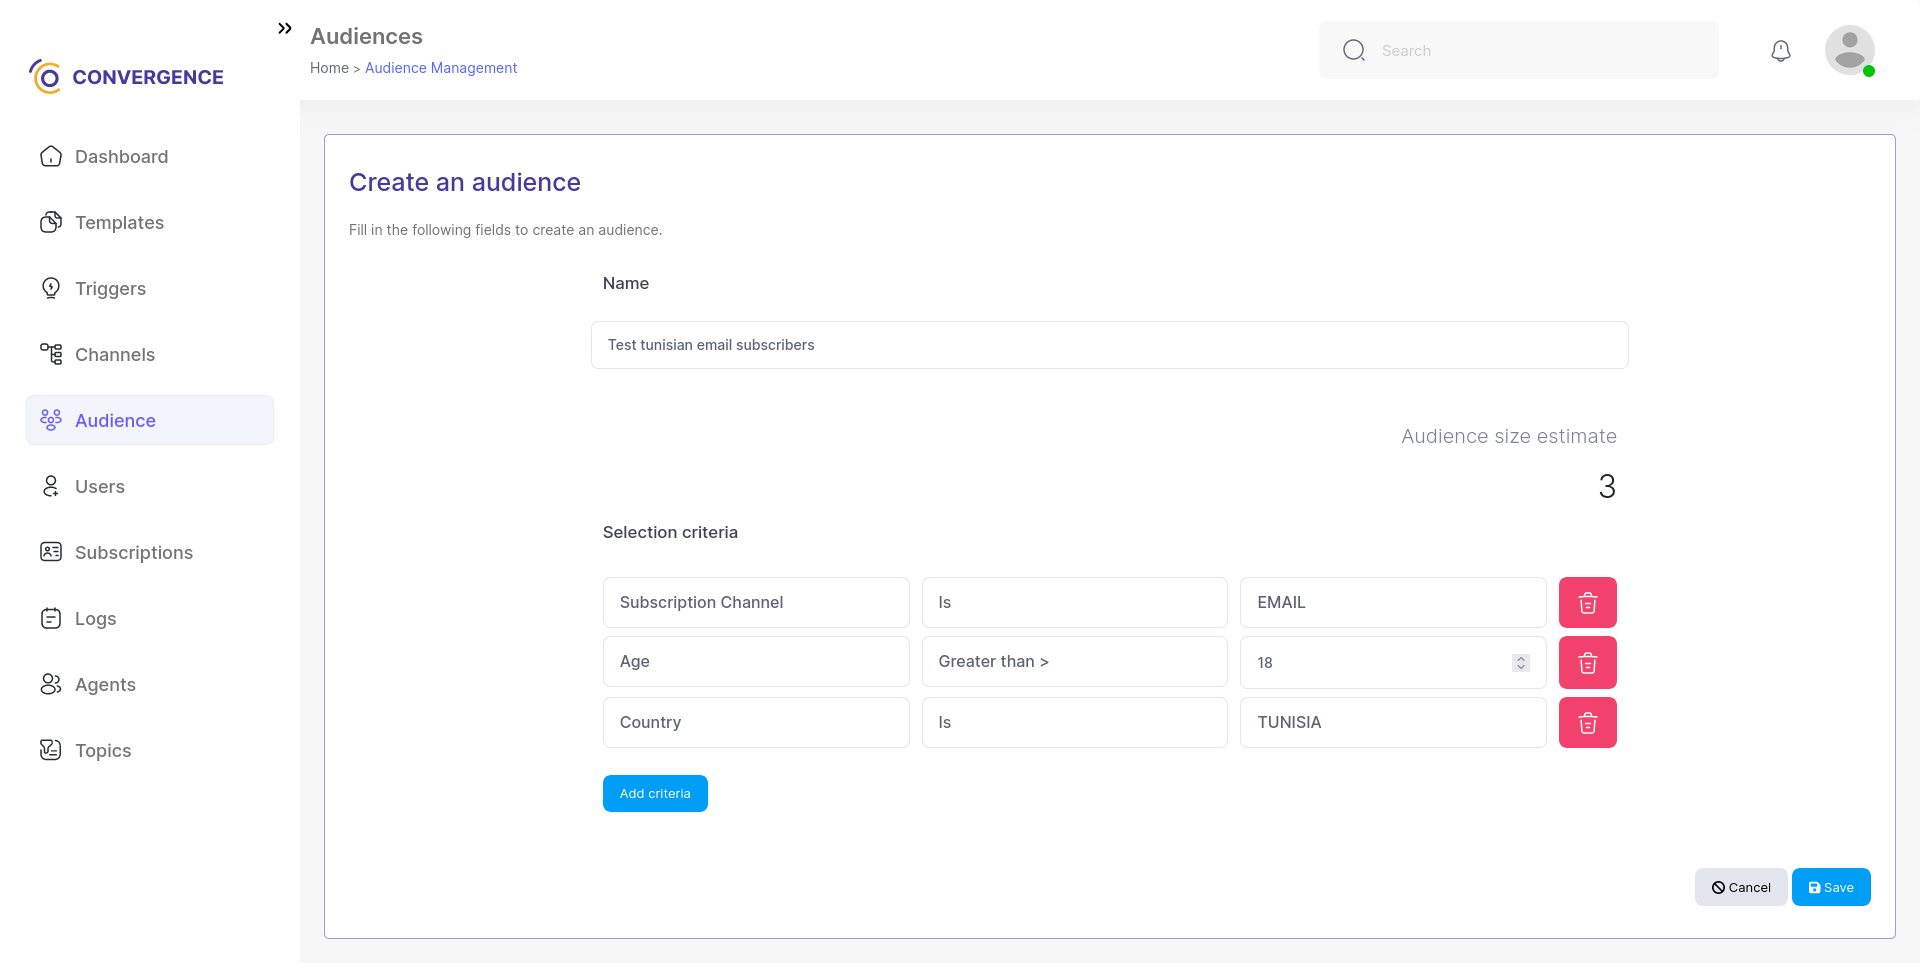
\includegraphics[width=\textwidth]{app/audience}
    \caption{Audience creation page}
    \label{ss-audience}
\end{figure}


\phantomsection
\section*{Summary}
\addcontentsline{toc}{section}{Summary}

In this initial release, we defined user stories and related constraints in the specification phase.
During the design phase we created a detailed plan that outlines how different components will interact to
ensure that the software is well-organized, efficient, and capable of addressing the intended needs and
goals. Finally, we showcased the result of implementing the essential components in our first release.

\noindent In the upcoming chapter, we will focus on the development of our second product release.